\documentclass[a4paper, 12pt]{article}
\usepackage[T2A]{fontenc}
\usepackage[utf8]{inputenc}
\usepackage[english,russian]{babel}
\usepackage{titletoc}
\usepackage{graphicx}
\usepackage{array}
\usepackage{etoolbox}
\usepackage{subfig}
\newcolumntype{P}[1]{>{\centering\arraybackslash}p{#1}}
\def\textunderset#1#2{\leavevmode
  \vtop{\offinterlineskip\halign{%
    \hfil##\hfil\cr\strut#2\cr\noalign{\kern-.3ex}
    \hidewidth\strut#1\hidewidth\cr}}}
\def\signhrule{\raggedright\baselineskip30.0ex \vrule height 0.5pt width30mm depth0pt}


\dottedcontents{section}[2.5em]{\bfseries}{2em}{0.5pc}
\dottedcontents{subsection}[3em]{}{2em}{0.5pc}

\usepackage{hyperref}
\hypersetup{
    colorlinks=true, %set true if you want colored links
    linktoc=all,     %set to all if you want both sections and subsections linked
    linkcolor=black,  %choose some color if you want links to stand out
}

\usepackage{verbatim}

\usepackage{listings}
\usepackage{xcolor}

\lstset
{%
	extendedchars=\true,
	inputencoding=utf8x,
	keepspaces=true,
	frame=tb,
	escapechar=|,
	xleftmargin=0.5cm,
	xrightmargin=0.5cm,
	columns=fullflexible,
	numbers=left,
	numbersep=4pt,
	showspaces=false,
	showstringspaces=false,
	breakatwhitespace=true,
	breaklines=true,
	basicstyle=\color{black}\small\sffamily,
	commentstyle=\color{gray}\itshape,
	stringstyle=\color{orange},
	numberstyle=\footnotesize\color{gray},
	keywordstyle=\color{blue}\bfseries,
	emphstyle={\color{blue}\bfseries},
	tabsize=2,
	texcl=true,
}

\lstdefinestyle{text}{
basicstyle=\small\ttfamily,
columns=flexible,
breaklines=true,
breakatwhitespace=true,
literate={\-}{{-\allowbreak}}1,
numbers=none,
postbreak=\mbox{\textcolor{red}{$\hookrightarrow$}\space},
}

\lstloadlanguages{SQL}

\newcommand{\Title}{Отчет о выполнении лабораторной работы}
\newcommand{\TaskType}{лабораторная работа}
\newcommand{\SubTitle}{по дисциплине <<Поддержка принятия решений в системах мониторинга>>}
\newcommand{\LabTitle}{Выявление логических закономерностей по данным мониторинга} 
\newcommand{\Faculty}{<<Информатика и системы управления>>}
\newcommand{\Department}{<<Компьютерные системы и сети (ИУ-6)>>}
\newcommand{\AuthorFull}{Козлов Владимир Михайлович}
\newcommand{\Author}{Козлов В.М.}
\newcommand{\Teacher}{}
\newcommand{\group}{ИУ6-13М}
\newcommand{\Year}{2024}
\newcommand{\Country}{Россия}
\newcommand{\City}{Москва}

\newcommand{\UpperFullOrganisationName}{Министерство науки и высшего образования Российской Федерации}
\newcommand{\ShortOrganisationName}{МГТУ~им.~Н.Э.~Баумана}
\newcommand{\FullOrganisationName}{федеральное государственное бюджетное образовательное учреждение высшего профессионального образования\newline <<Московский государственный технический университет имени Н.Э.~Баумана (национальный исследовательский университет)>> (\ShortOrganisationName)}

\textwidth=163mm
\textheight=220mm
\oddsidemargin=-0.5pt
\footskip=30pt
\topmargin=27pt
\headheight=12pt
\headsep=25pt
\topskip=10pt
\baselineskip=15pt
\topmargin=-4mm
\begin{document}
\vspace*{-\baselineskip}
\vspace*{-\headheight}
\vspace*{-\headsep}
\vspace*{-2pt}
\thispagestyle{empty}
\begin{center}

% Шапка
{\centering
\begin{tabular}{P{0.15\textwidth}P{0.85\textwidth}}
\smash{
		\raisebox{-0.9\height}{
		
\includegraphics[width=0.15\textwidth]{includes/bmstu.pdf}
		}}
 & \UpperFullOrganisationName\newline \FullOrganisationName \\
\hline
\multicolumn{1}{p{0.15\textwidth}}{} & \multicolumn{1}{p{0.85\textwidth}}{} \\
\multicolumn{1}{p{0.15\textwidth}}{ФАКУЛЬТЕТ}	&	\multicolumn{1}{p{0.85\textwidth}}{\Faculty}	\\
\multicolumn{1}{p{0.15\textwidth}}{КАФЕДРА}	&	\multicolumn{1}{p{0.85\textwidth}}{\Department}	\\
\end{tabular}}
\vfil

{% Основная часть
\vfil
\Large
\underline{\MakeUppercase{\Title}}
\newline
\SubTitle
\vfil
\large
\begin{tabular}{p{0.3\textwidth}p{0.5\textwidth}} 
	Студент:	& \AuthorFull \\ 
	\hline
	Группа:	& \group \\ 
	\hline
	Тип задания:	& \TaskType \\ 
	\hline
	Тема:	& \LabTitle \\ 
	\hline
	\end{tabular}

\vfil

\begin{tabular}{p{0.45\textwidth}p{0.25\textwidth}P{0.25\textwidth}} 
\large
Студент	&	\textunderset{\scriptsize{подпись, дата}}{\signhrule} & \textunderset{\scriptsize{Фамилия, И.О.}}{\ifdefempty{\Author}{\signhrule}{\underline{\Author}}} \\ 
& & \\
Преподаватель	&	\textunderset{\scriptsize{подпись, дата}}{\signhrule} & \textunderset{\scriptsize{Фамилия, И.О.}}{\ifdefempty{\Teacher}{\signhrule}{\underline{\Teacher}}} \\ 
\end{tabular}
}

\vfil
\vfil
\City, \Year

\end{center}

\pagebreak
\tableofcontents
\newpage
% Основная часть --------------------------------------------------------------------------------------------
\section*{Цель}
\addcontentsline{toc}{section}{Цель}
Изучение методов интеллектуального анализа данных, необходимых для разработки алгоритма принятия решения в условиях неопределенности.
\section*{Задание}
\addcontentsline{toc}{section}{Задание}
При выполнении лабораторной работы необходимо формализовать задачу принятия решения по распознаванию текущего образа в системе мониторинга, разработать алгоритм распознавания и классификации образа, реализовать интеллектуальный подход при принятии решения в условиях неопределенности. Затем необходимо составить отчет по лабораторной работе с полученными результатами.
\newpage
% -------------------------------------------------------
\section{Выполнение работы}
\subsection{Исходные данные}
Были выбраны следующие эталонные символы
\begin{center}
  \centering
  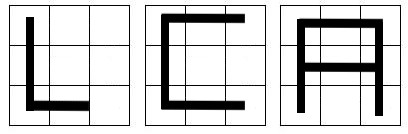
\includegraphics[width=.7\linewidth]{extra/input.jpg}
  \captionof{figure}{Эталонные символы}
  \label{fig:prplot}
\end{center}
И следующий тестовый символ.
\begin{center}
  \centering
  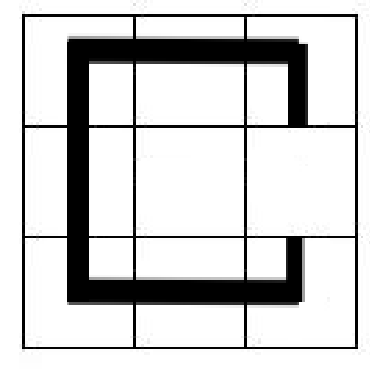
\includegraphics[width=.3\linewidth]{extra/test.png}
  \captionof{figure}{Эталонные символы}
  \label{fig:prplot}
\end{center}
Единицами были переведены в вектора из двоичных чисел в разрядах которых зашифрованы касания краёв клетки по порядку: левая, верхняя, правая, нижняя.
\lstinputlisting[language=Python, caption=Представление векторов]{../data_extended.py}
Для конвертации векторов в векторы чисел, их центрирования и нормирования, а также поиска сопряжённых векторов использовались следующие функции:
\lstinputlisting[language=Python, caption=Вспомогательные функции]{../lib.py}
Непосредственно классификация образа происходила в следующем скрипте:
\lstinputlisting[language=Python, caption=Скрипт классификации образа]{../main.py}
\lstinputlisting[style=text, caption=Вывод скрипта классификации образа]{extra/output.txt}
Результат решения дифференциальных уравнений представлен на следующем рисунке:
\begin{center}
  \centering
  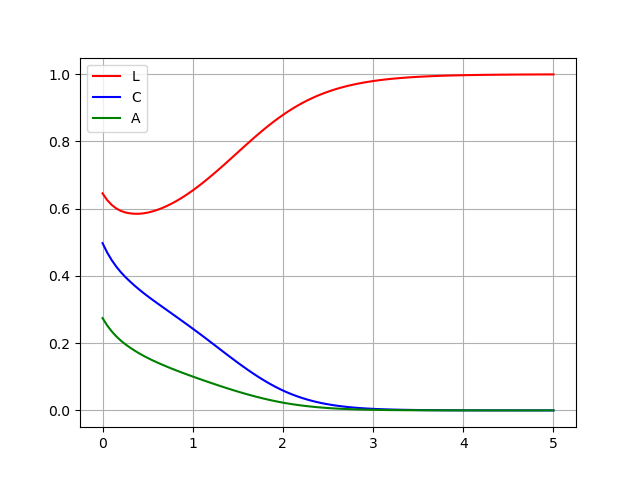
\includegraphics[width=.7\linewidth]{extra/output.png}
  \captionof{figure}{Результат решения дифференциальных уравнений}
  \label{fig:prplot}
\end{center}
Как видно на изображении был распознан символ С, что является верным.
\newpage
% -------------------------------------------------------
\section{Ответы на вопросы}
\subsection*{Вопросы}
\begin{enumerate}
  \item Что понимают под процессом принятия решений в системах мониторинга?
  \item Почему решения в системах мониторинга принимают в условиях неопределенности? Поясните ответ.
  \item Что понимают под неопределенностью информации?
  \item Поясните технологию Data Mining, ее цели и задачи?
  \item Укажите основные этапы интеллектуального анализа данных;
  \item Поясните задачу классификации объектов. Чем она отличается от задачи кластеризации?
  \item С какой целью организуют защиту данных в системах мониторинга?
\end{enumerate}
\subsection*{Ответы}
\begin{enumerate}
  \item Это этап обработки данных, когда система принимает меры или вырабатывает рекомендации на основе анализа информации, собранной из различных источников.
  \item Решения в системах мониторинга принимаются в условиях неопределенности, поскольку данные, собираемые из различных источников, могут быть неполными, неточными или подверженными шуму. Например, состояние оборудования может быть связано с множеством переменных, многие из которых могут изменяться или быть неизвестными. Кроме того, данные, поступающие от датчиков, могут содержать погрешности или интерпретироваться по-разному, что добавляет неопределенность в процесс принятия решений.
  \item Неопределенность информации относится к ситуации, когда данные, собранные с датчиков, устройств или других источников, не полностью точны, неполны или содержат неопределенные элементы.
  \item Data Mining — это процесс извлечения полезных знаний и закономерностей из больших объемов данных с использованием статистических, математических и алгоритмических методов. Цели включают выявление скрытых паттернов, прогнозирование и принятие решений. Задачи — классификация, кластеризация, регрессия и ассоциация данных.
  \item Основные этапы интеллектуального анализа данных включают:
    \begin{enumerate}
      \item Определение цели анализа.
      \item Сбор и подготовка данных.
      \item Применение алгоритмов анализа.
      \item Оценка и интерпретация результатов.
      \item Принятие решений.
      \item Обратная связь и улучшение моделей.
    \end{enumerate}
  \item Задача классификации объектов заключается в назначении метки или категории объектам на основе их признаков, используя обучающие данные с известными метками. Кластеризация, в отличие от классификации, не требует заранее заданных меток и заключается в группировке объектов по схожести, выявляя скрытые структуры в данных.
  \item Защита данных в системах мониторинга организуется с целью обеспечения конфиденциальности, целостности и доступности информации.
\end{enumerate}
\newpage
%---------------------------------------------------------
\section{Вывод}
При выполнении лабораторной работы был применён алгоритм распознавания и классификации образа и реализован интеллектуальный подход при принятии решения в условиях неопределенности.
\end{document}
